\documentclass{article}
\usepackage{amsmath}
\usepackage[style=authoryear]{biblatex}
\usepackage{graphicx}
\usepackage[]{hyperref}
\usepackage{tabularray}
\usepackage{siunitx}
\usepackage[noabbrev]{cleveref}
\addbibresource{bib/PhD.bib}
\begin{document}

\author{\and{Luke Thomas Smith} \and{Eun-Jung Holden} \and{Tom Horrocks} \and{Daniel Wedge} \and{Naveed Akhtar}}
\title{Magnetic grid resolution enhancement using machine learning: A case study from the Eastern Goldfields Superterrane}
\date{2022-09-21}
\maketitle{}

\begin{abstract}
    Densely sampled geophysical surveys are a key driver for mineral exploration, but sample density, and therefore grid resolution, is limited by survey cost.
    Consequently, computational methods are resorted to for upsampling, or `super-resolving', of gridded geophysical survey data.
    However, existing approaches such as interpolation filters do not leverage high-resolution detail from pre-existing geophysical surveys.
    Through the application of state-of-the-art deep learning super-resolution architectures, accurate high-resolution grids are predicted from corresponding low-resolution grid priors.
    Specifically, the RDN and ESRGAN+ neural network architectures, which were originally developed for enhancing images, are applied to enhance magnetic surveys and trained with high-resolution and low-resolution magnetic grids of the same extent.
    \SI{80}{\metre} cell size magnetic grids are upsampled to \SI{20}{\metre} cell size using this method, and predicted value and structural accuracy comparisons to the corresponding ground truth \SI{20}{\metre} grids are presented over two test sites in the Eastern Goldfields Superterrane, Western Australia.
    The method based on RDN achieves 53\% lower error compared to Bicubic interpolation.
    The case study demonstrates that the deep learning approach can improve the resolution and frequency content of geophysical surveys without requiring additional sampling expense, while remaining accurate against known ground truth surveys.
    Super-resolution may assist in the interpretation of low-resolution survey grids, however these upsampled grids cannot perfectly recreate the accuracy of highly sampled surveys gridded at their optimal cell size.
\end{abstract}

\section{Introduction}
\subsection{Resolution in geophysics}
\label{resingeo}
Surveys of the spatial distribution of physical properties of the Earth, such as the magnetic potential field, are common in geoscience.
These point-sampled surveys are typically interpolated onto a grid raster, and when a raster covers a known spatial extent, its resolution can be referred to as spatial resolution, indicating that each pixel covers a quantified area.
Often referred to as high resolution, a fine spatial resolution is critical for representing high frequency components in a gridded raster.
These high frequency components reveal localised variations in the surveyed potential field, which provide additional detail on subsurface geological structures and the potential for mineralisation.
An example of the additional detail provided by a high-resolution grid is provided in \cref{lrandhr}, which shows an \SI{80}{\metre} cell size Total Magnetic Intensity (TMI) grid (a) compared to a \SI{20}{\metre} TMI grid of the same \SI{2560}{\metre} \texttimes\ \SI{2560}{\metre} extent (b), gridded from the same potential field samples, but interpolated to different resolutions.
The increased density of pixels in the high-resolution \SI{20}{\metre} grid allows higher frequencies in the sampled magnetic potential field to be displayed.
These frequencies are irretrievably lost when the high-resolution grid is downsampled to \SI{80}{\metre}.

\begin{figure}[hbt]
    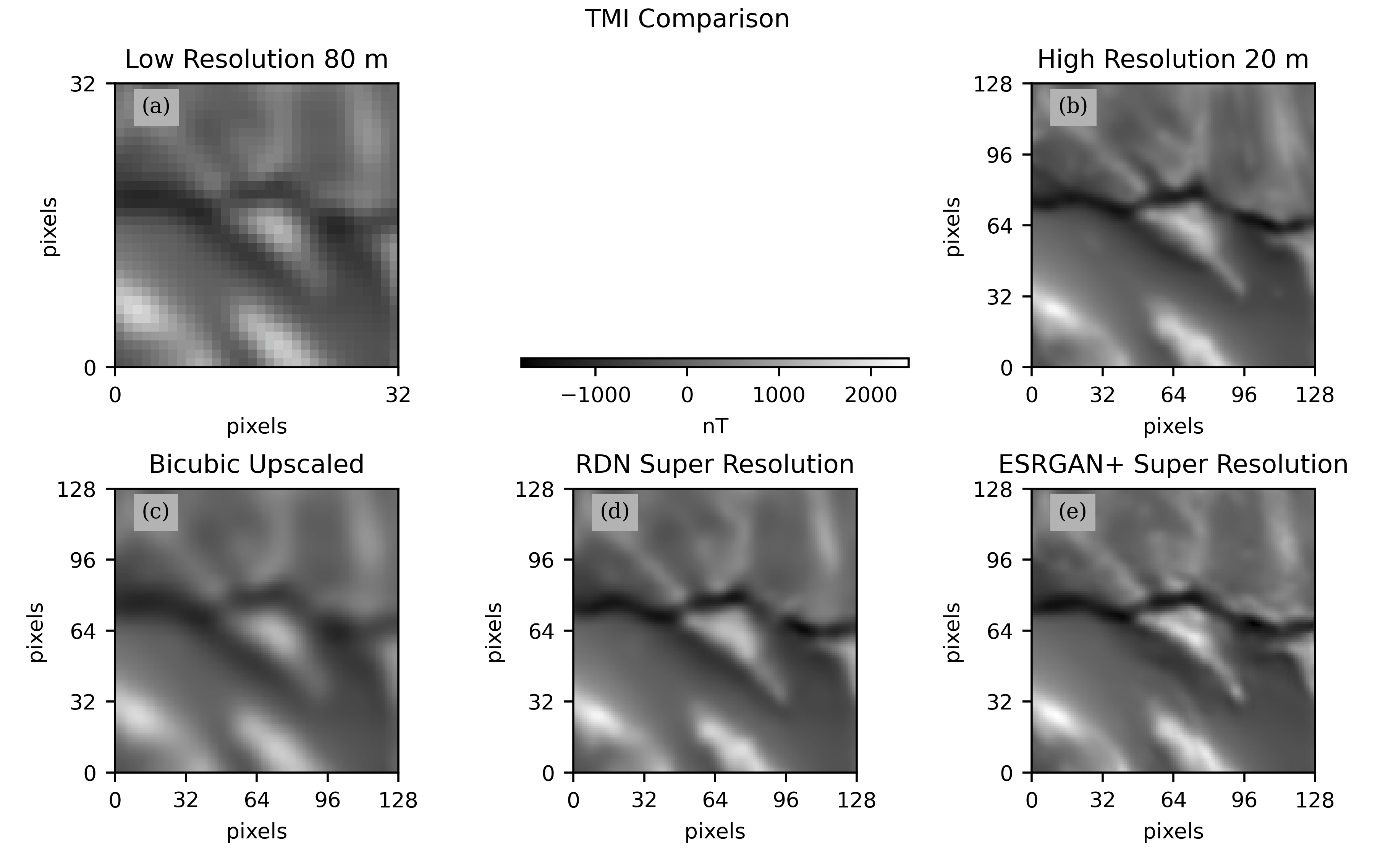
\includegraphics[width=\textwidth]{fig/p1/image1.png}
    \caption[Comparison of different resolution grids]{Low resolution \SI{80}{\metre} cell size (a), and high-resolution \SI{20}{\metre} cell size (b) TMI grids over the same extent.
    Each tile is \SI{2560}{\metre} \texttimes\ \SI{2560}{\metre}.
    The additional detail shown in the high-resolution grid is made available by the finer cell size, which can convey higher frequency detail, if present in the sampled data.}
    \label{lrandhr}
\end{figure}

Geophysical rasters are created through a process of survey point sampling, grid interpolation, and usually post-process filtering.
During these processes, the sampled potential field may be subject to destructive Nyquist sampling principles \parencite[16]{dentithGeophysicsMineralExploration2014}, especially due to the original point sampling interval and the cell size (pixel spatial extent) selected for the grid interpolation.
The optimal grid cell size is dependent on the sampling interval, and because of this, the highest frequency component preserved in gridded geophysical potential fields is intrinsically limited by the original sampling interval.
This could be summarised as; high frequency components that may be sampled in surveys with close line sampling will be preserved in high-resolution grids with fine cell size.
Typically, cell sizes as fine as one fifth of the line sampling interval can be useful for gridding airborne geophysics \parencite{reidAeromagneticSurveyDesign1980}.
Selecting a cell size finer than one fifth will increase the number of pixels in the image raster, achieving a higher resolution, however no additional geophysical frequencies exist in the point sampled data to be displayed and no detail will be gained.

\subsection{Resolution and frequency}
As discussed in \cref{resingeo}, a finer spatial resolution grid (fewer metres per pixel) can convey higher frequency information, due to the higher spatial sampling rate.
Indeed, a gridded raster with regularly spaced square cells $\Delta x$ has an intrinsic Nyquist wavelength $\lambda _N$, at twice the cell size \labelcref{eq:nyq}.

\begin{equation}
    \lambda N = 2 \Delta x
    \label{eq:nyq}
\end{equation}

This corresponds to the shortest wavelength the grid can adequately display, which can be observed as the finest details resolvable in the grid raster.
For example, a high-resolution grid with \SI{20}{\metre} spatial resolution (HR) has a Nyquist wavelength of \SI{40}{\metre}.
In comparison, a low-resolution \SI{80}{\metre} grid (LR) has a Nyquist wavelength of \SI{160}{\metre}.
Note the Nyquist wavelength is proportional between different cell size grids according to the scale factor S \labelcref{eq:hrn}.

\begin{equation}
    \lambda N_{HR} = \lambda N_{LR} \div S
    \label{eq:hrn}
\end{equation}

Because the highest frequency component preserved in a grid is limited by the grid cell size, any operation that coarsens the cell size is a low pass filter.

\subsection{Improving resolution}
Given the value of higher detail when viewing images, there has been significant research into improving image resolution.
The most straightforward method is to simply sample at a higher rate, which for airborne geophysics means increasing the density of line sampling over a given area.
However, increasing sampling density increases total sampling cost, and cannot easily be done for existing grids.
This paper will investigate a new method for enhancing the resolution of grids by predicting high frequency components in geophysics without requiring additional sampling or cost, based on machine learning methods for image super-resolution.

Recent advances in machine learning techniques for image super-resolution (SR) have been shown to successfully increase image resolution for photographs and other image rasters, while also improving perceptual image quality.
These modern techniques belong to a family of methods known as deep learning, where features learnt early in the network are leveraged to develop a higher understanding of later features.
Notable published examples include SRCNN \parencite{dongLearningDeepConvolutional2014}, VDSR \parencite{kimAccurateImageSuperresolution2016}, SRGAN \parencite{ledigPhotorealisticSingleImage2017}, EDSR \parencite{limEnhancedDeepResidual2017}, RDN \parencite{zhangResidualDenseNetwork2018}, and the current state-of-the-art methods, ESRGAN \parencite{wangESRGANEnhancedSuperResolution2018} and ESRGAN+ \parencite{rakotonirinaESRGANFurtherImproving2020}.
SRGAN and ESRGAN are similar in design to their contemporary counterparts but implement a Generative Adversarial Network (GAN) framework.
In a GAN framework, the upsampling network (termed generator) is trained in an adversarial manner against another network (termed discriminator).
Adversarial training of upsampling networks can help in learning a better model for the task at hand.
For example, ESRGAN uses an analogous upsampling network design to RDN (Residual Dense Network) \cref{fig:rdn}, with the addition of a discriminator network.
This will be further discussed in \cref{sec:nnsr}.
For a review on super-resolution networks, the reader is referred to \cite{anwarDeepJourneySuperresolution2020}.

Neural network based super-resolution has seen recent success across many scientific disciplines on data other than natural images.
It is popular in satellite remote sensing \parencite[e.g.][]{lanarasSuperresolutionSentinel2Images2018,wangUltradenseGANSatellite2019}, and has been applied to astrophysics \parencite[e.g.][]{jungbluthSingleframeSuperresolutionSolar2019,salvatelliUsingUNetsCreate2019}, fluid dynamics \parencite{bodeUsingPhysicsinformedEnhanced2021}, elevation models \parencite{leongDeepBedMapDeepNeural2020}, hyperspectral data \parencite[e.g.][]{arunCNNBasedSuperResolutionHyperspectral2020}, and seismic geophysics data \parencite[e.g.][]{liDeepLearningSimultaneous2021,wangDeeplearningbasedSeismicData2018,wangAdaptingResidualDense2022,yuDeepLearningDenoising2019}.
These authors typically report a lower error between the super-resolution upsampled product and ground truth data when compared to a bicubic upsampled product and the ground truth data, as well as improved perceptual quality.
Critically, super-resolution for these applications was able to create realistic high frequency information during upsampling, which could be validated against existing high-resolution surveys of the same extent.
While there are pre-trained models to super-resolve image data (such as ImageNet), the smooth and continuously differentiable nature of potential field data makes it difficult to directly apply such pre-trained models.
For example, it may enhance the appearance of gridding artifacts, instead of supressing them.
While several of the aforementioned works investigate deep learning super-resolution for geospatial data, low resolution in potential field geophysics is a result of under sampling and naïve best-effort interpolation of the potential field, distinct from low-resolution data previously studied in those works.

\begin{figure}
    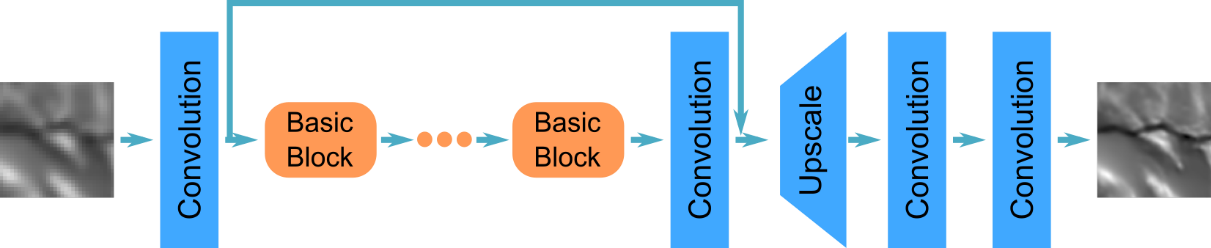
\includegraphics[width=\textwidth]{fig/p1/image2.png}
    \caption[The RDN architecture]{The RDN architecture, which acts as the ESRGAN generator.
    Twenty-three Basic Blocks are stacked sequentially to form the main convolution path.
    Upsampling to the target output size is performed after the main convolution sequence.
    Adapted from \cite{wangESRGANEnhancedSuperResolution2018}.
    }
    \label{fig:rdn}
\end{figure}

Resolution enhancement in potential field geophysics (occasionally referred to as downward continuation in this context) is performed numerically.
\cite{chenPotentialFieldData2022} use Taylor series expansion, while \cite{xuGravityAnomalyReconstruction2019} interpolate randomly sampled gravity point data using the nonequispaced Discrete Fourier Transform (nDFT), which leverages compressed sensing theory \parencite{candesIntroductionCompressiveSampling2008}.
While high quality results from under sampled data are attained with the non-equispaced Discrete Fourier Transform, the grid line sampling methodology of airborne geophysical surveys is highly regular, and unlikely to satisfy the coherency constraints required for compressive sensing.
This maintains true for data from published grids, which are regularised onto a uniform grid.
To the best of our knowledge, detailed studies on applying and comparing deep learning approaches for geophysical potential field super-resolution has not been previously reported.

\begin{figure}[hbt]
    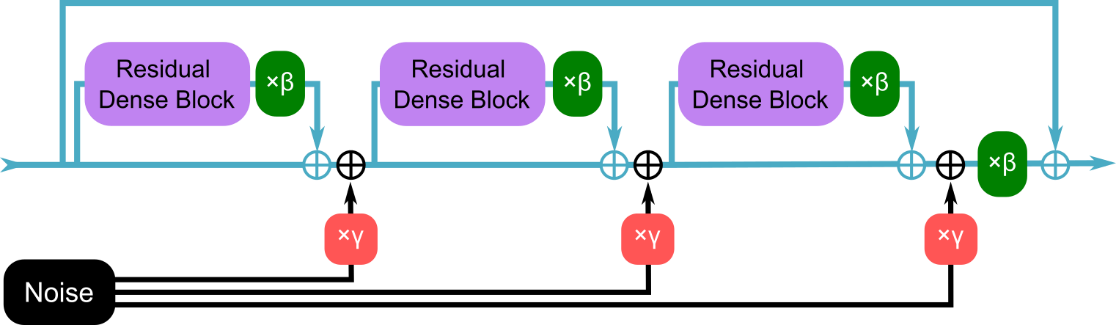
\includegraphics[width=\textwidth]{fig/p1/image3.png}
    \caption[Basic Blocks]{Each Basic Block (\cref{fig:rdn}, orange) comprises three weighted Residual Dense Blocks (\cref{fig:convs}).
    ESRGAN+ extends ESRGAN with the addition of Gaussian Noise after each basic RDB block (black vectors).
    Weight factors are indicated by $\beta$ and $\gamma$.
    Noise injection is not used in RDN\@.
    Adapted from \cite{rakotonirinaESRGANFurtherImproving2020}.
    }
    \label{fig:rdb}
\end{figure}

\begin{figure}[hbt]
    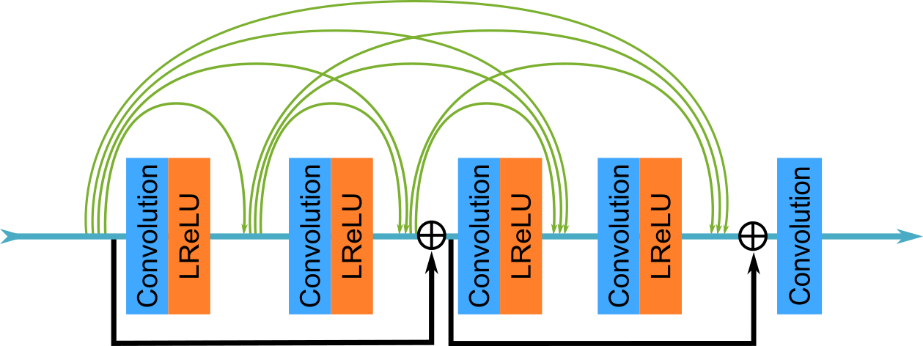
\includegraphics[width=\textwidth]{fig/p1/image4.png}
    \caption[RDB convolutional layers]{Each Residual Dense Block (\cref{fig:rdb}, purple) comprises four convolutional layers, with additional learning pathways present as residual connections (black), and dense connections (green).
    LReLU refers to the Leaky-ReLU activation function.
    Adapted from \cite{rakotonirinaESRGANFurtherImproving2020}.
    }
    \label{fig:convs}
\end{figure}

\subsection{Interplation}
Increasing the resolution of an image is achievable through computationally inexpensive interpolating filters, such as nearest neighbour or bicubic interpolation.
These algorithms increase the number of pixels comprising the image raster and predict values for the interpolated pixels.
The nearest neighbour algorithm makes a simple prediction that the value of an interpolated pixel is equal to the nearest ground truth pixel, while the bicubic filter predicts values at interpolated pixels using a cubic function fit to the neighbouring ground truth pixels.
Bicubic interpolation results in a smoothing effect \parencite{keysCubicConvolutionInterpolation1981}, which means it is of limited value for adding higher frequencies to geophysics without additional input data.
It is however suitable as a baseline method to compare upsampling performance against deep learning methods.
It is typical for super-resolution algorithms to use a nearest neighbour upsampling step during their process to achieve the desired output image size, but the upsampled grid is subsequently processed by the neural network to incorporate additional information.
Importantly, basic interpolation is capable of increasing the number of pixels in a grid, but has limited predictive power for high frequency components.
Simply selecting a finer cell size when gridding line sampled data is likely to equal or outperform post-gridding interpolation.

\subsection{Neural network super-resolution}
\label{sec:nnsr}
Convolutional neural network (CNN) upsampling methods use features learned during their training to accurately upscale novel features during inference on novel data.
Learning from an extensive and varied training dataset is a primary driver for the improved performance of CNN methods over simple interpolation methods.
We apply the architectures of two CNN techniques in this work for geophysics super-resolution.
Namely, ESRGAN+ \parencite{rakotonirinaESRGANFurtherImproving2020} which exploits a GAN framework, and a non-GAN variant of the same method which does not rely on the discriminator component of the GAN framework.
The latter has a close resemblance to Residual Dense Network \parencite{zhangResidualDenseNetwork2018} in its architecture.
These CNN models are designed for natural images containing three channel inputs, whereas magnetic and other scientific grids use single channel floating point values.
Hence, for each network it was necessary to change the input array channel count from 3 to 1, and adjust the normalisation method to suit magnetic anomaly values.
We compare these methods to bicubic interpolation to demonstrate the predictive power of the deep learning approaches.

Residual Dense Network (RDN) \parencite{zhangResidualDenseNetwork2018} is a deep learning super-resolution method which consists of a series of residual dense blocks (\cref{fig:rdb,fig:convs}), which combine the performant residual connections and dense connections (\cref{fig:convs}) of earlier architectures for state-of-the-art performance.
Residual and dense connections provide additional learning capacity to a CNN, where features learnt in early layers can be fully utilised in later layers.
Following a series of these residual dense blocks, image enlargement is achieved using a simple nearest neighbour interpolation process followed by additional convolution operations.
In this case, enlargement is performed on an intermediate representation of the input, which has gained information during the main network path.
RDN is trained to reduce the Mean Absolute Error L1-norm loss, which corresponds to minimising the absolute difference between the super-resolution prediction and the high-resolution ground truth grid.
RDN was selected as a comparison against ESRGAN+ because RDN is structurally similar to the generator network in ESRGAN, allowing for analysis of the performance of GANs for super-resolution geophysics.
The RDN implementation used here adopts some improvements from ESRGAN+ and will henceforth be referred to as RDN\textdaggerdbl{}.

ESRGAN+, based on ESRGAN \parencite{wangESRGANEnhancedSuperResolution2018}, was chosen as the primary super-resolution CNN architecture for this task due to its reported success in other super-resolution tasks (especially \cite{bodeUsingPhysicsInformedSuperResolution2019} and \cite{leongDeepBedMapDeepNeural2020}) and state of the art results for its original application in image super-resolution.
As a Generative Adversarial Network (GAN), it comprises two iteratively trained neural networks, a Generator (G) used to upscale low-resolution inputs, and Discriminator (D), which is trained to improve the performance of the generator.

G is analogous in design to the RDN architecture described above (\cref{fig:rdn}), and is trained to upscale a low-resolution input, creating a super-resolution prediction.
The Discriminator network used in ESRGAN is based on a prevalent image classification architecture known as VGG \parencite{simonyanVeryDeepConvolutional2015}.
D is trained to classify its inputs as being either an example of the super-resolved G prediction, or high-resolution ground truth data.
This is used to provide a loss-feedback to G based on G's ability to create realistic SR predictions.
The two networks are trained concurrently, with the contemporaneous D network being used to calculate an adversarial loss for G at each iteration.
The adversarial loss calculated by D is incorporated with the generator's L1 loss as used in RDN, and training continues until D stabilises at 50 \% accuracy where the discriminator is unable to distinguish generated images from real images better than random chance.
At this point, training has converged, and the trained generator model can be used to independently upscale novel inputs.

The specific variant of ESRGAN applied in this work is that of ESRGAN+ \parencite{rakotonirinaESRGANFurtherImproving2020}, which incorporates modern GAN performance improving techniques, including generator noise injection (noted in \cref{fig:rdb}), and additional dense and residual connections (noted in \cref{fig:convs}).
These additional connections are used in RDN\textdaggerdbl{}.

The prediction of grid cell values for interpolation is common practice in geophysics.
Existing methods, including nearest neighbour and bicubic filtering, have limited capacity to predict high frequency details to incorporate in upsampled grids, limiting the amount of detail these grids can capture and display.
Recent super-resolution machine learning methods have demonstrated capacity to accurately predict high frequency components in grids from a variety of scientific disciplines, and application of these methods to geophysical potential fields will be investigated here.

\section{Materials and Methods}
\subsection{Geophysical context}
The Eastern Goldfields Superterrane of Western Australia is extensively covered by aeromagnetic surveys of \SI{400}{\metre} line spacing or better, especially over its South-Western extent.
Large survey extents are government sponsored through the Exploration Incentive Scheme \parencite[e.g.][]{griffinStimulatingGreenfieldsExploration2010}, with these low-resolution regional surveys serving to identify prospective areas to undertake surveys at higher resolution.
A number of these higher resolution surveys have been publicly released to open file.
In the Eastern Goldfields the driver for this extensive magnetic coverage is the prominence of highly susceptible BIF and ultramafic formations, which host several major resource projects including Mt Mason (iron ore), Mt Ida and Comet Vale (gold/silver), and Goongarrie (nickel/copper).
A long geological history provides our test region with a variety of magnetic features and textures to test super-resolution performance with, including structurally complex high intensity formations (BIF and ultramafic units), broad textural regions (granites), and extensive linear features (dykes).
Shear zones and fault systems provide further variation to these structures.
Overall, the selected test region in the Eastern Goldfields Superterrane contains sufficient variety of features on which to examine the effect and value of super-resolution upsampling, and determine the suitability of the method for application in other regions.

\subsection{Data}
In typical image SR networks, training data typically take the form of image pairs; the original high-resolution (HR) image, and a low-resolution (LR) image generated on-the-fly by bicubically downsampling the HR image, typically at a scale factor of four.
A similar technique could be used in geophysics SR by applying a low pass filter with a suitable cut-off to a HR grid to simulate the LR counterpart.
However, here we use data from existing grids published at the appropriate four times resolution difference, namely the Magnetic merged grid of Western Australia 2020 at \SI{20}{\metre} (HR) and \SI{80}{\metre} (LR) cell sizes \parencite{brett80MagneticMerged2020}.
When these grids were created, the best available resolution of all grids across the state were compiled at \SI{20}{\metre} cell size, and interpolated to \SI{80}{\metre} using a 4th order Newton polynomial interpolation process \parencite[][personal communication]{brett80MagneticMerged2020}.
This is similar to bicubic interpolation, in that both methods are examples of localised polynomial based interpolation algorithms.
While the cell size is uniform for each respective state grid, the sampling interval of the contributing line surveys varies across the state, which affects the extent of coverage of high frequency components across each grid.
To ensure that the HR ground truth has additional high frequency detail to the LR during training, data were only selected from areas of the Goldfields area of the state grid with contributing survey line spacing \SI{300}{\metre} or closer (optimal cell size strictly finer than \SI{80}{\metre}).
Training and validation data were extracted independent to a reserved test area, outlined in \cref{fig:trainvaldata}.
By selecting mixed line spacing data in this way, transforms between different scales of frequency loss are captured in the training data.
That is, the same model can learn from fine optimal cell size extents that lose many component frequencies when interpolated to \SI{80}{\metre}, as well as coarse cell size extents which may only lose few or none.
These data were extracted as square tiles, each covering \SI{2560}{\metre} by \SI{2560}{\metre} at 32 \texttimes{} 32 pixels for LR, and 128 \texttimes{} 128 pixels for HR, with no overlap.
This resulted in \num{5290} training tile pairs (used to train the model), \num{512} validation tile pairs (used to select the best performing model), and \num{2415} test tile pairs (used to independently verify the performance of the selected model).
These magnetic grid tiles differ notably from standard colour image tiles, in that they contain 32-bit floating-point values in a single channel, corresponding to the TMI value at each grid cell location.
These values were min-max scaled to a range of 0 to 1 using the global minimum and maximum values of the HR training data.
In summary, the single channel high- and low-resolution state TMI grids were filtered according to a database of their component surveys to extract areas of \SI{300}{\metre} line spacing or less.
These data were normalised according to the statistics of the HR training set, and split into small patches suitable for the hardware limitations.
After application of the architecture under investigation, the data are returned to predicted TMI values, and recompiled into a contiguous spatial extent.

\begin{figure}[]
    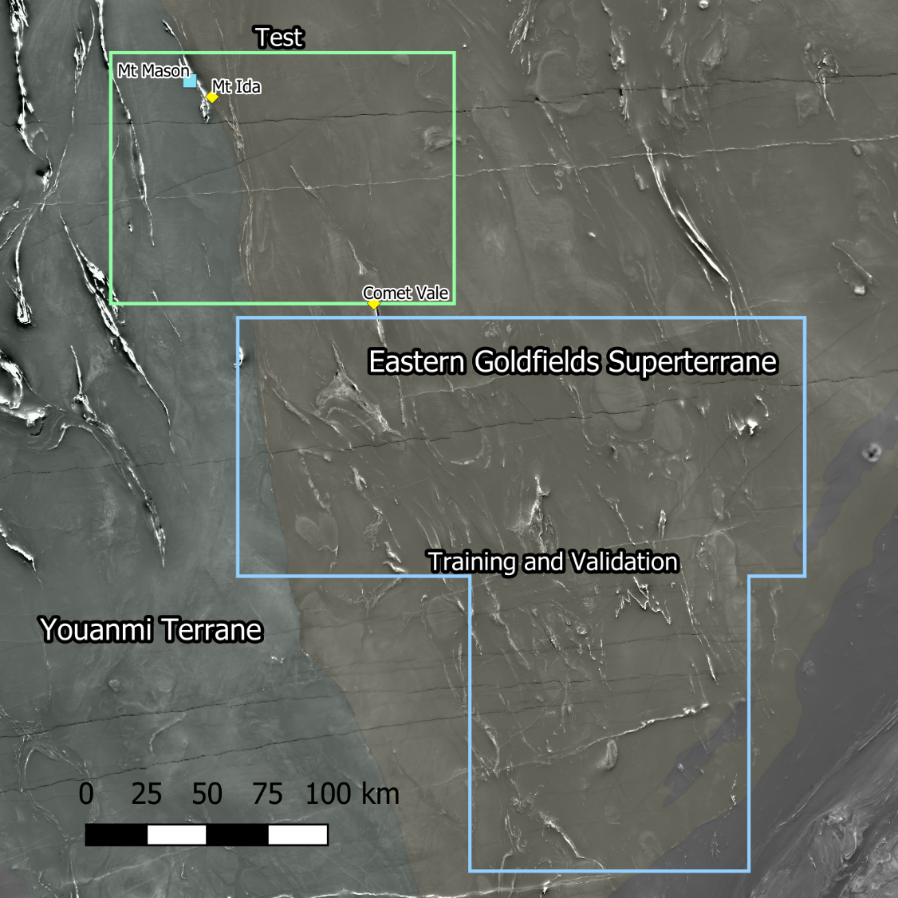
\includegraphics[width=\textwidth]{fig/p1/image5.png}
    \caption[Dataset context]{Reserved training/validation and test areas of Eastern Goldfields Superterrane magnetic grid, and their tectonic context.
    Background: \SI{20}{\metre} merged magnetic grid of Western Australia, \parencite{brett40MagneticMerged2020}.
}
    \label{fig:trainvaldata}
\end{figure}

\subsection{Training and inference implementation}
Training of the RDN\textdaggerdbl{} and ESRGAN+ networks was performed with Pytorch \parencite{paszkePyTorchImperativeStyle2019} using an Nvidia RTX 3090 with 24 GB memory, on a desktop computer with an Intel i9-10900KF CPU and 64 GB RAM\@.
Both networks were trained with minibatch size of 64 image patch pairs for \num{602} epochs (\num{17.6} h for RDN\textdaggerdbl{}, \num{21.8} h for ESRGAN+), at which point the PSNR plateaued.
Training samples were augmented using random 90-degree rotations and flips to encourage a model with rotational and symmetrical invariance to the input images, and their order per epoch was shuffled to improve regularisation and supress overfitting.
Further measures for the suppression of overfitting inherent to each of the applied architectures are described in their respective manuscripts \parencite{wangESRGANEnhancedSuperResolution2018,zhangResidualDenseNetwork2018}.
The optimiser used was Adam \parencite{kingmaAdamMethodStochastic2015}.
The learning rate was adjusted over the course of the experiment using the Pytorch implementation of One Cycle Learning Rate scheduler \parencite{smithSuperconvergenceVeryFast2018}, which provides a “warm up” period to stabilise early predictions, and a “cool down” period where the loss minima is fine tuned.
Following the generator implementation from ESRGAN+, twenty-three Residual Dense Blocks were ordered sequentially to form the main network, followed by two nearest neighbour upsampling filters at two times scale each.
The ESRGAN+ discriminator followed that of \cite{rakotonirinaESRGANFurtherImproving2020} which is an implementation of a VGG style classification network \parencite{simonyanVeryDeepConvolutional2015}.
For ESRGAN+ the peak learning rate was \num{6e-4}, and the feature loss, pixel loss (MAE), and adversarial loss parameters were weighted at \num{1}, \num{0.01}, and \num{0.005} respectively.
RDN\textdaggerdbl{} had a peak learning rate of \num{3e-4} and did not require loss component weighting because only L1 pixel loss is used.
Bicubic interpolation was carried out using the implementation provided in Pillow \parencite{vankemenadePythonpillowPillow2021}, a ubiquitous open source Python imaging library.
Inference is carried out using the frozen weights of the trained upsampling models, and takes approximately \num{0.1} s per 32 \texttimes{} 32 pixel tile.
Inference is performed on a tiled basis due to the size of input grids being too large for GPU RAM, and the results may be patched together for full extent visualisation and analysis, or displayed as single tiles.
Predicted outputs are inverse normalised to return the cell values to appropriately scaled TMI units.

\subsection{Accuracy Metrics}
The functional aim of super-resolution geophysics is to accurately predict realistic high frequency details to add to a low-resolution grid.
To quantify this, we calculate root mean square error (RMSE) and structural similarity metrics (SSIM and MS-SSIM), on TMI, high pass filtered TMI, and first vertical derivative (1VD) filtered TMI results for each upsampling method across several sample extents.
Euclidean accuracy measures like RMSE quantify the per-pixel accuracy of a predicted grid compared to its corresponding high-resolution ground truth grid.
For this metric, quality improves as the error value approaches \num{0}.
The Structural Similarity (SSIM) \parencite{wangImageQualityAssessment2004} and Multi-Scale Structural Similarity (MSSSIM) \parencite{wangMultiscaleStructuralSimilarity2003} image quality metrics use sliding windows to quantify image perceptual similarity based on localised structural information.
MS-SSIM extends SSIM by performing a weighted sum of the measure at several different scales.
In both structural metrics, the result is a combination of localised image luminance, contrast, and structural information.
A SSIM value of 1 indicates perfect similarity, and values approaching 0 indicate increasing dissimilarity.

\section{Results}
Results are presented to compare the three methods described above, with the metrics of RMSE, SSIM and MS-SSIM, as well as observed perceptual quality.
In addition to unfiltered TMI comparisons, high pass filtered and first vertical derivative TMI grids are also shown.
These products are commonly used in geophysics to investigate high frequency components in grids.

\subsection{Test dataset}
We first present a visual comparison of a selected feature rich \SI{80}{\metre} cell size LR tile, its counterpart \SI{20}{\metre} HR ground truth tile, and the result of; the bicubic upscaling filter, the RDN\textdaggerdbl{} upsampling network, and the ESRGAN+ upsampling network as applied to the LR tile (\cref{fig:resultsvis}).
This tile was selected from the reserved test region in the Eastern Goldfields Superterrane, and neither of the low- or high-resolution samples were seen during training.
The result of bicubic interpolation (\cref{fig:resultsvis} c) demonstrates the smoothing effect of the bicubic filter, while the Residual Dense Network (\cref{fig:resultsvis} d) and ESRGAN+ network (\cref{fig:resultsvis} e) show added detail.
The two neural network methods more closely match the ground truth \SI{20}{\metre} tile than the bicubic upsampled image does, when observing feature edges and textural detail.


\begin{figure}
    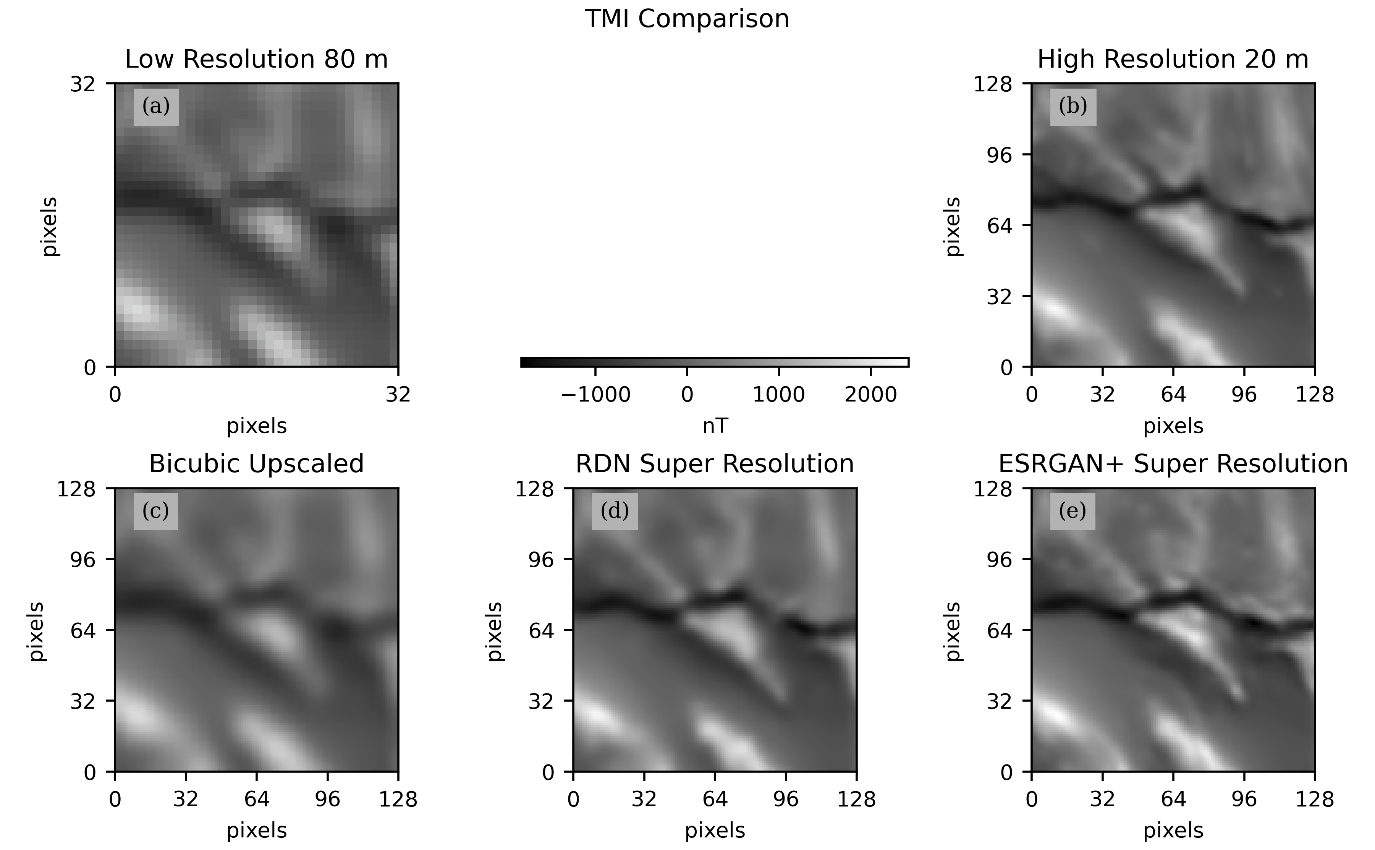
\includegraphics[width=\textwidth]{fig/p1/image6.png}
    \caption[Visual inference results]{Visual comparisons of a selected tile from the reserved test region.
    The \SI{80}{\metre} low-resolution input (a) is shown at equivalent size to the \SI{20}{\metre} high-resolution ground truth (b) using nearest neighbour interpolation.
    The colourmap is shared between subfigures.
    }
    \label{fig:resultsvis}
\end{figure}

\Cref{fig:residuals} demonstrates the error residuals between the predicted TMI grids for each upsampling method and the HR ground truth.
For the selected tile, the RMSE is best minimised using RDN\textdaggerdbl{}, which also shows the best structural metric performance.
ESRGAN+ outperforms the bicubic method in RMSE and MSSIM\@.

\begin{figure}
    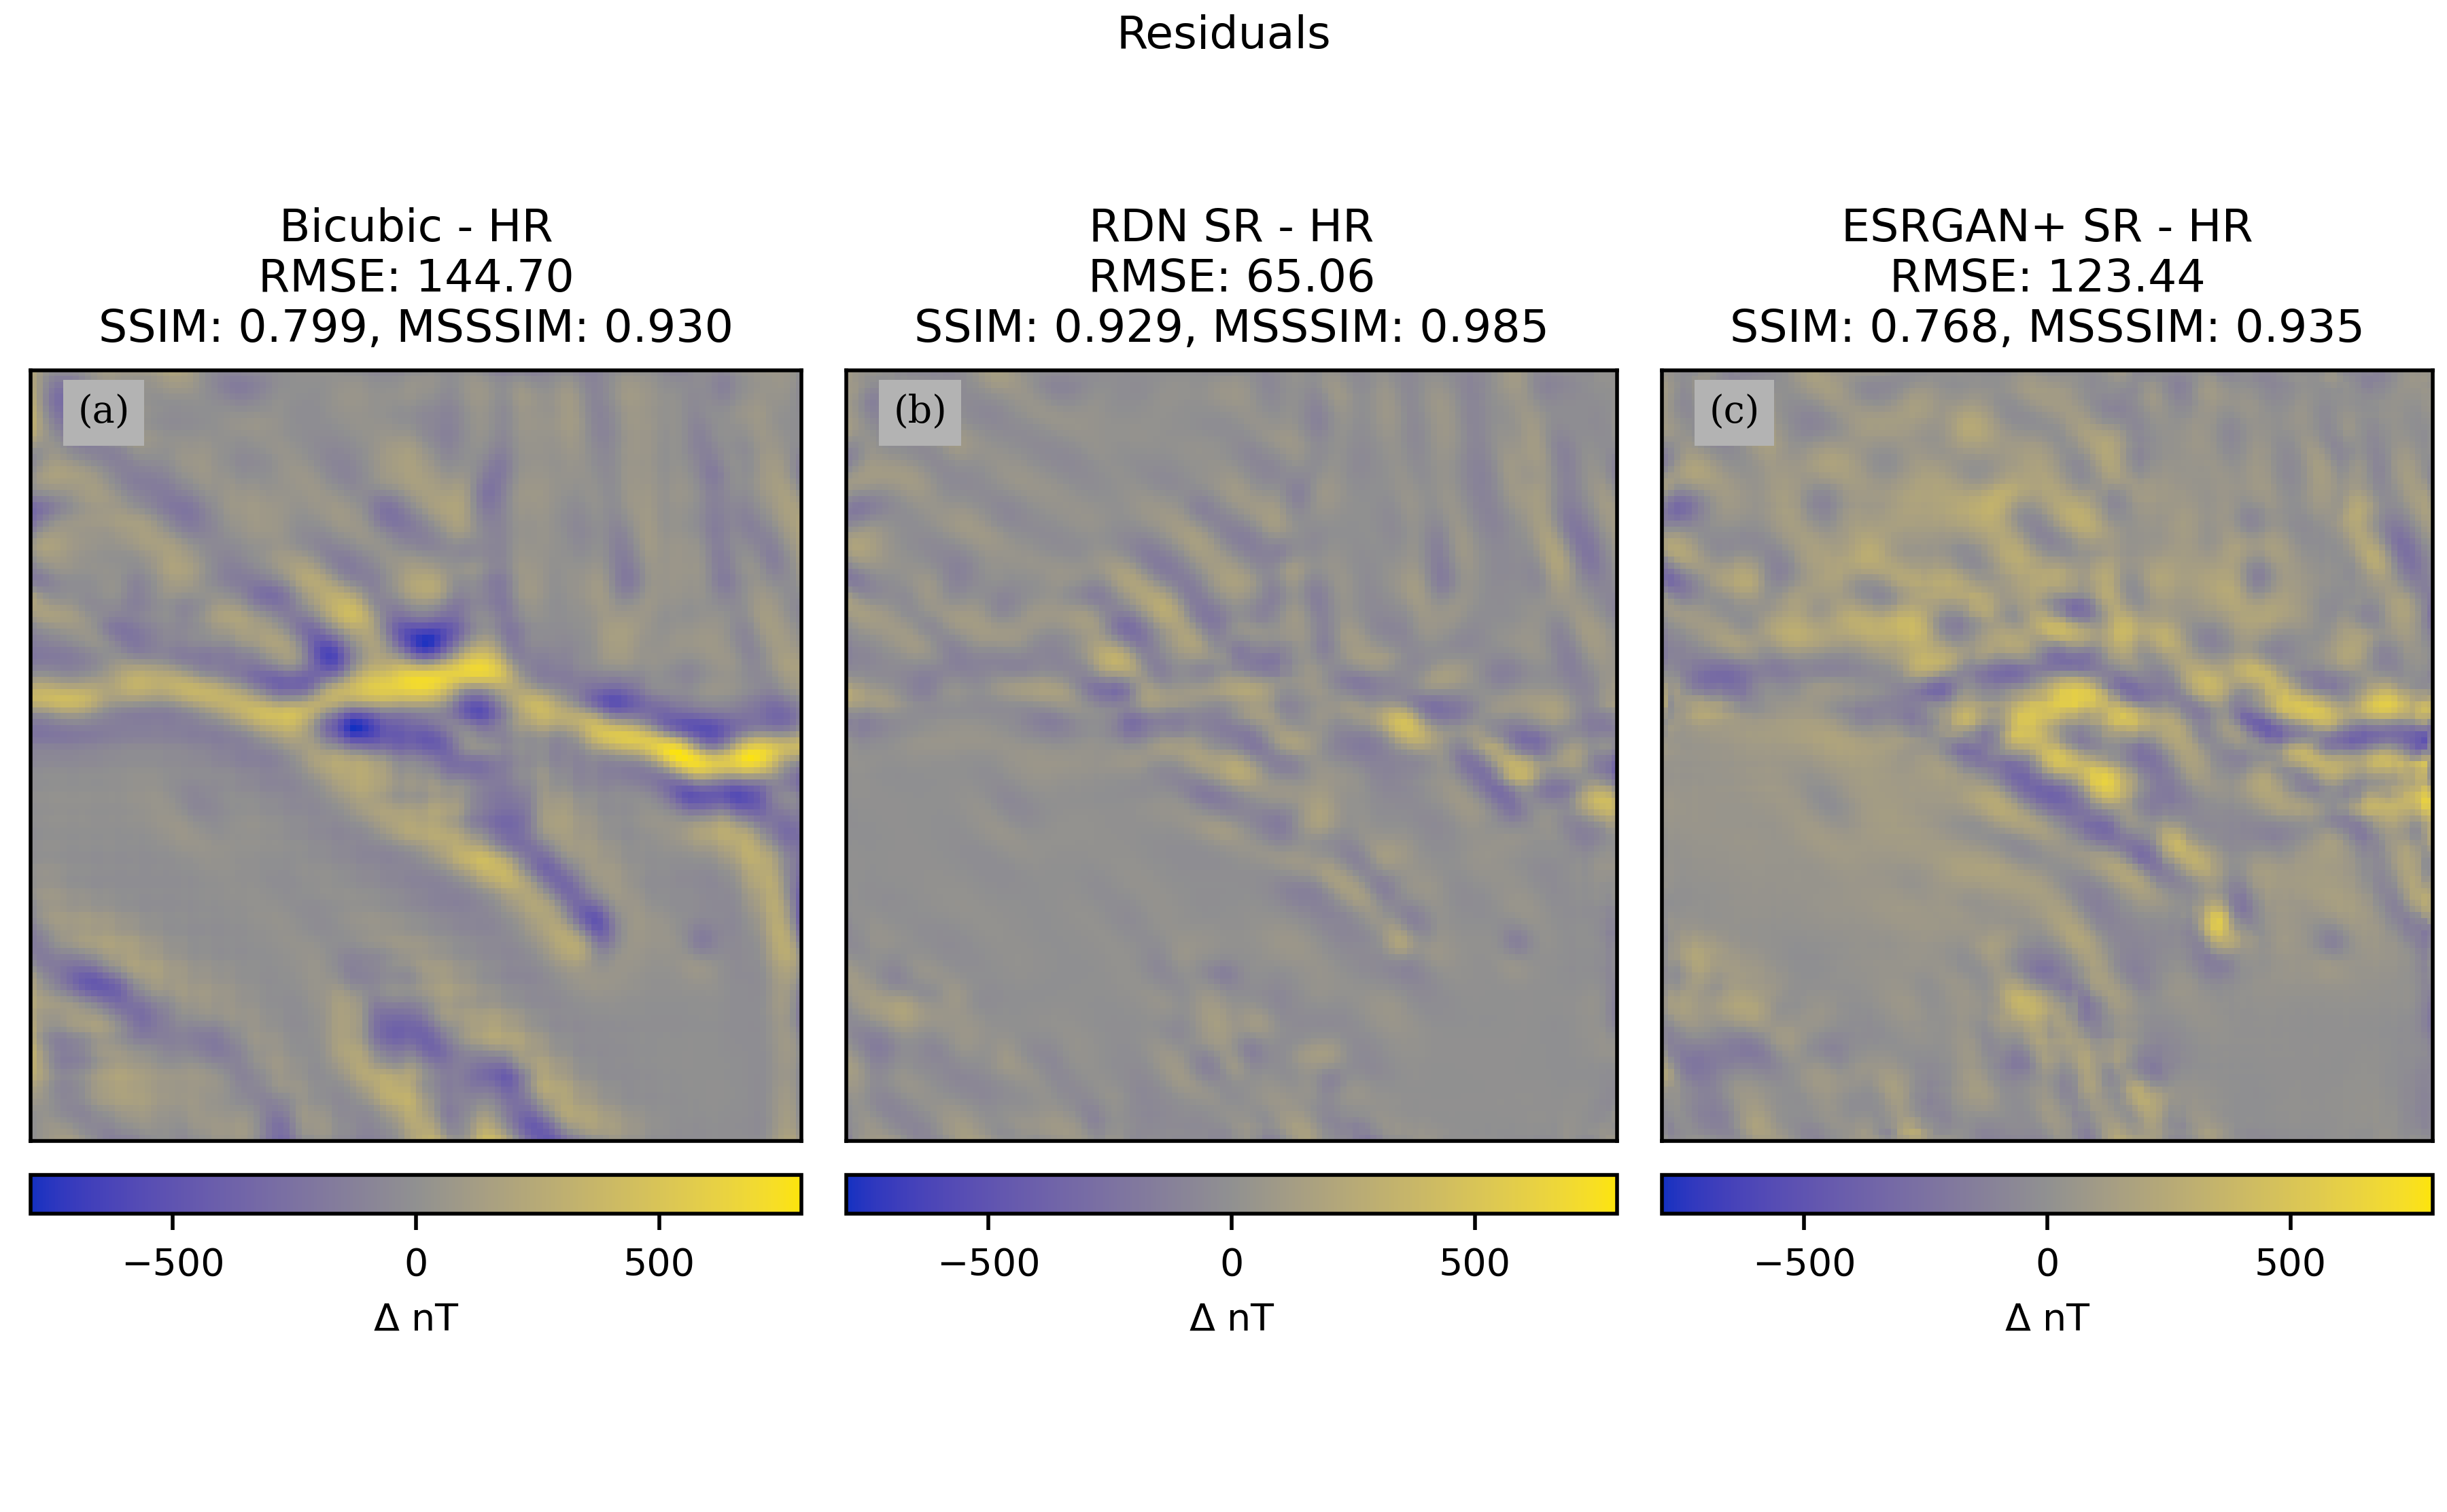
\includegraphics[width=\textwidth]{fig/p1/image7.png}
    \caption[Error residuals map for a selected tile]{Error residuals map for the selected test tile, for each upsampling method; Bicubic (a), RDN\textdaggerdbl{} (b), and ESRGAN+ (c).
    Image quality metrics are reported for each upsampled tile, calculated against the groundtruth HR\@.}
    \label{fig:residuals}
\end{figure}

The prediction of higher frequencies can be quantified using the Radially Averaged Power Spectral Density.
In the Fourier domain, the amplitudes of an array's component frequencies are mapped to coordinates representing their orientation.
The Radially Averaged Power Spectral Density (RAPSD) \parencite{ulichneyDitheringBlueNoise1988} is a one-dimensional representation of the cumulative power of each frequency component, in any orientation within the image.
\cref{fig:rapsd} shows the RAPSD for the different methods over the test extent shown in \cref{fig:trainvaldata}. The deep learning methods have consistently superior power in predicted wavelengths between approximately \SI{640}{\metre} and \SI{120}{\metre}, with RDN\textdaggerdbl{} closely matching the groundtruth spectra, while ESRGAN+ tends to exaggerate.

% TODO USE REVISED MANUSCRIPT FIGURES 

\begin{figure}
    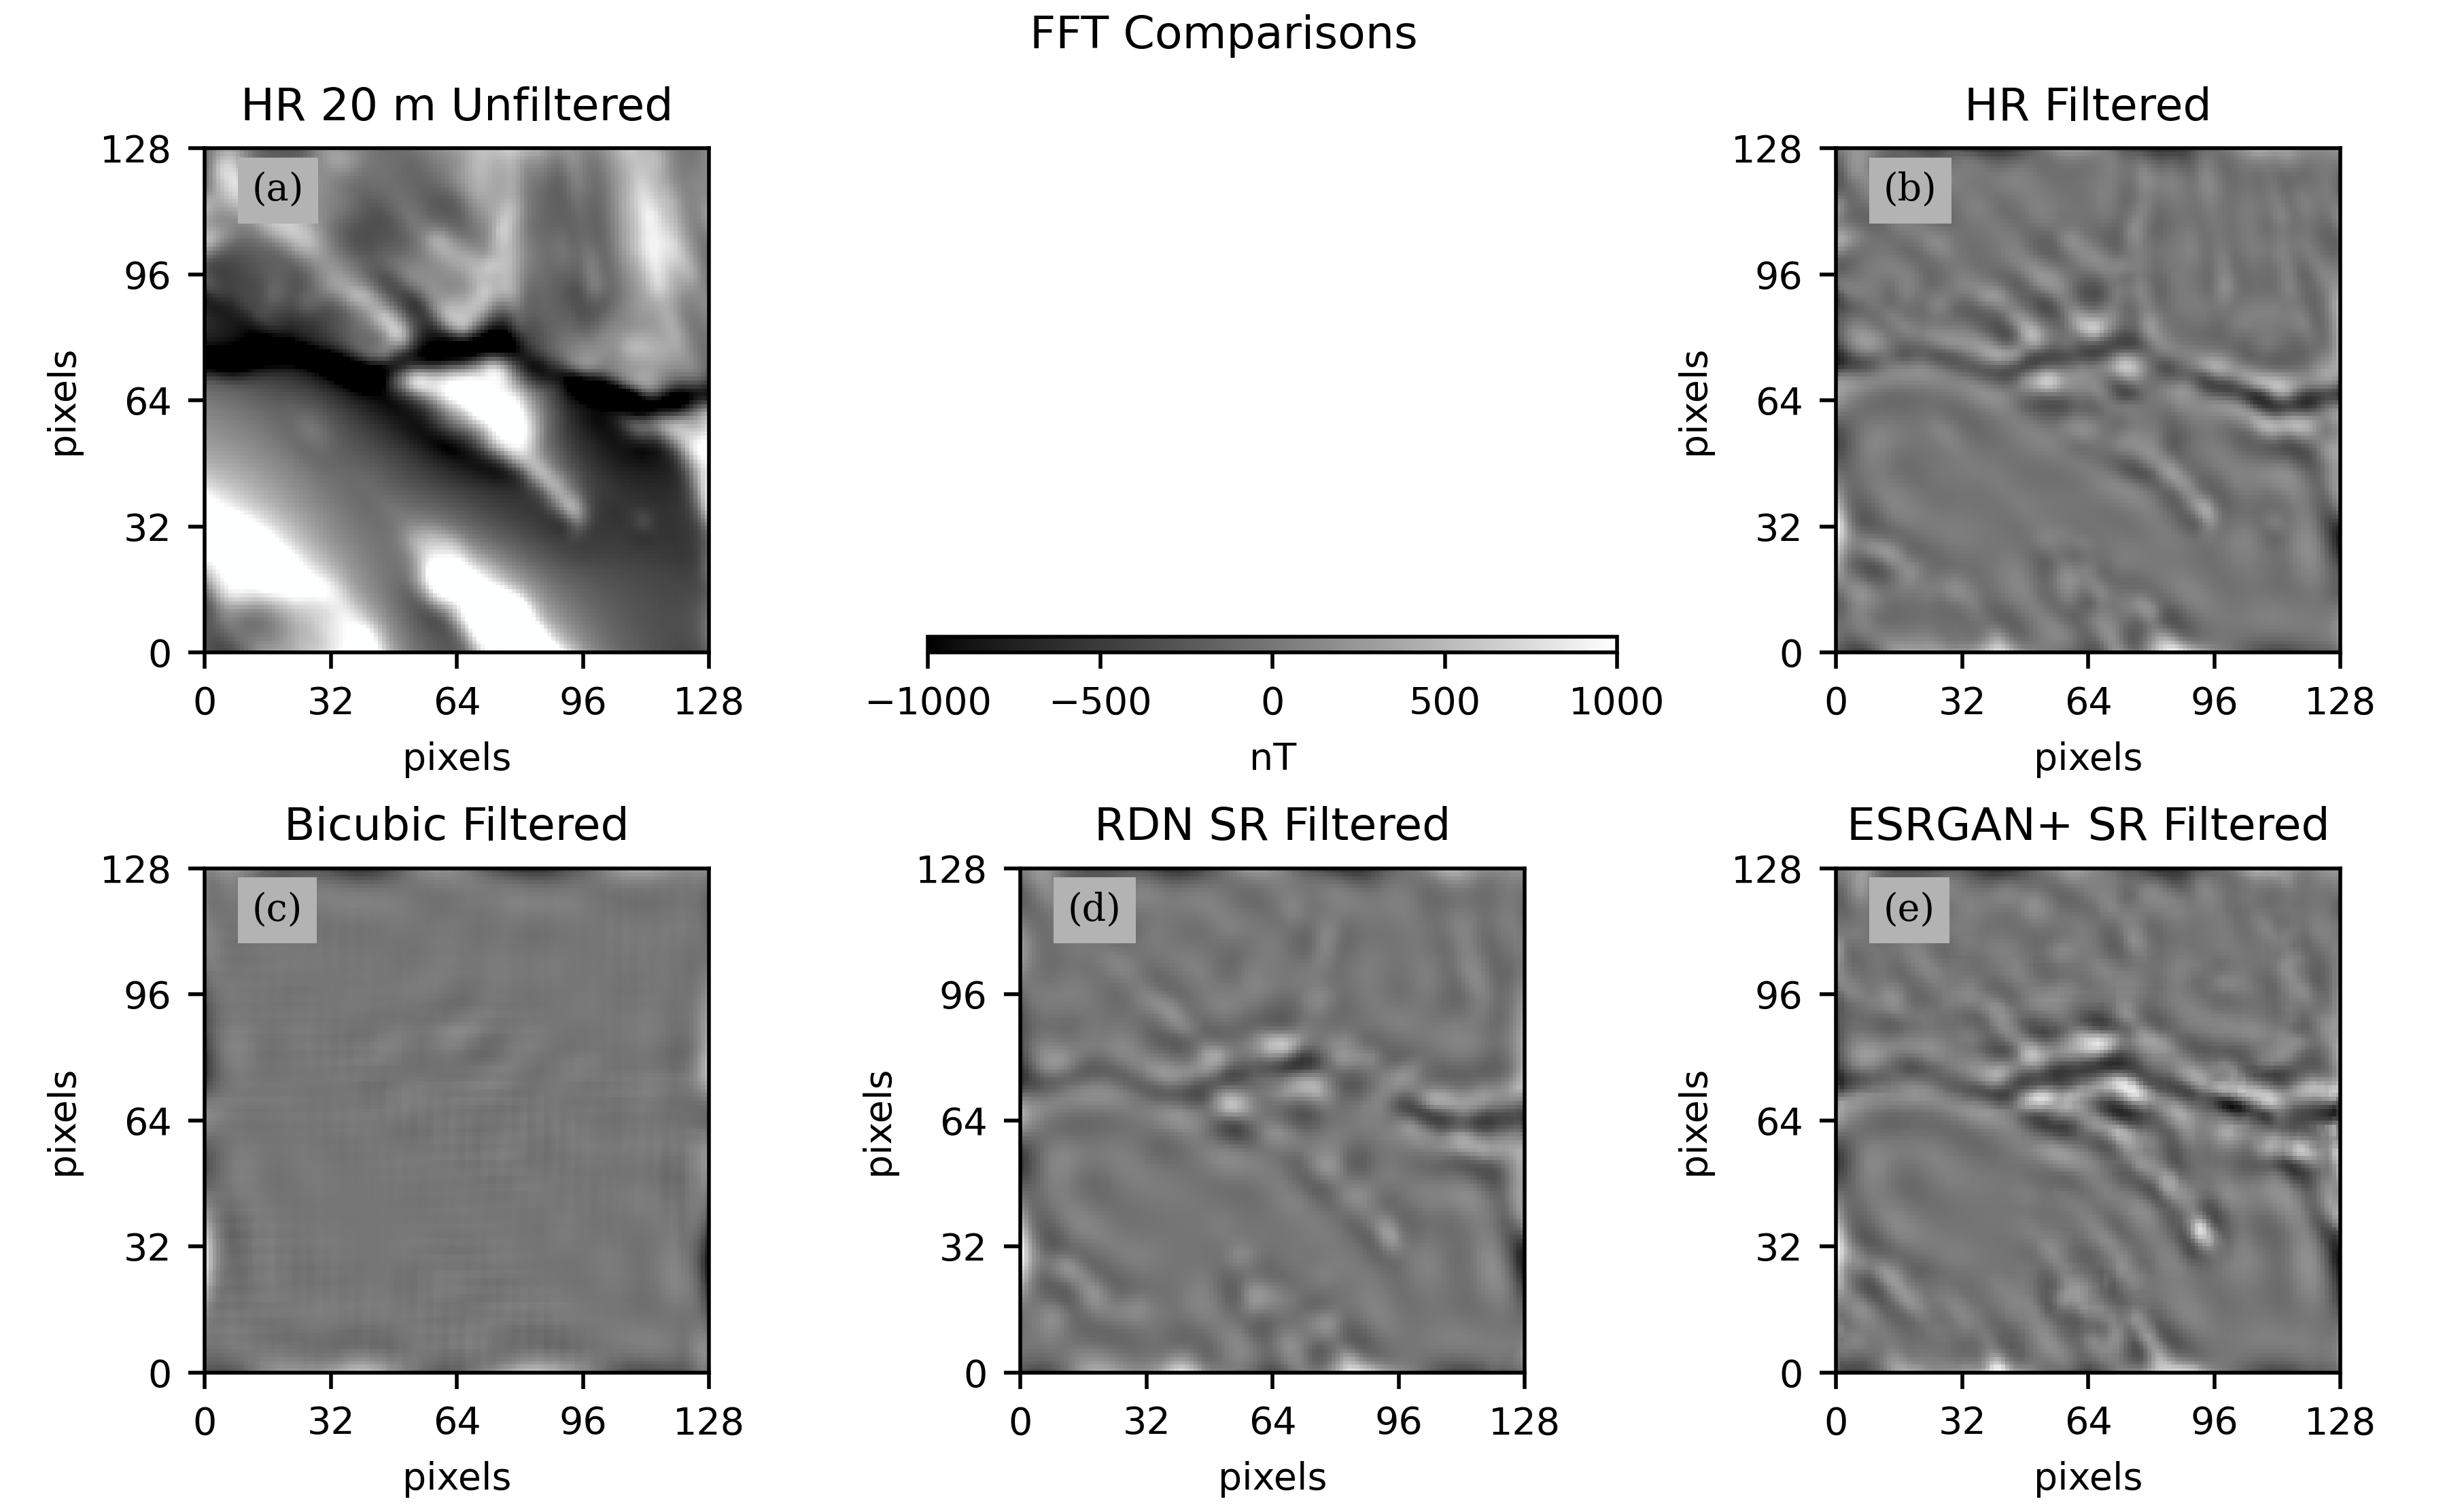
\includegraphics[width=\textwidth]{fig/p1/image8.png}
    \caption[short]{Radially Averaged Power Spectra for the complete test extent shown in \cref{fig:trainvaldata}.
    The Nyquist wavelengths for the high-resolution (and upsampled) rasters and low-resolution raster are also shown.
    The frequency axis has been transformed to wavelength, and the spectra have been normalised for direct comparison.
    Note the complete test extent is covered by surveys with a range of line spacings from \SI{100}{\metre} to \SI{20}{\metre}, with \SI{100}{\metre} being the most extensive.
    The Nyquist wavelength of the \SI{100}{\metre} surveys (optimal grid cell size approximately \SI{20}{\metre}) likely causes the reduction in power at \SI{55}{\metre} and \SI{220}{\metre}.
    }
    \label{fig:rapsd}
\end{figure}

To visualise the contribution of these enhanced high frequencies in the resulting grid, the super-resolved output from each method is high pass filtered, with a cut-off wavelength equivalent to the Nyquist wavelength of the LR grid.
By filtering at this wavelength, only frequencies added by the upsampling process will be shown in the output (\cref{fig:filtered}). Bicubic interpolation (\cref{fig:filtered} c) fails to add significant high frequency components.
RDN\textdaggerdbl{} (\cref{fig:filtered} d) appears to approximate similar high frequencies to the HR tile (\cref{fig:filtered} b), while ESRGAN+ (\cref{fig:filtered} e) shows potentially excessive predicted high frequency components.
Finally, metrics for the full set of test tiles are reported in \cref{tab:metrics}.
The non-GAN CNN approach of RDN\textdaggerdbl{} remains the most accurate method for the entire test grid.
Several routinely occurring artefacts are observed in the two super-resolution products, especially in ESRGAN+ which incorporates details it has learned from the Discriminator network loss.
The First Vertical Derivative filter is used in \cref{fig:jhillvis} to demonstrate the ability to perform common geophysical filters on super resolved grids, and to emphasise examples of these artefacts.
The most apparent artefact arises from the inference implementation when upsampling a grid larger than fits in memory, where visible edges appear around individual tiles in the compiled inference grid (e.g. \cref{fig:jhillvis}, *).
This could be reduced by adjusting the size of inference tiles, or slightly overlapping adjacent input tiles.
Predictions from ESRGAN+ commonly show a ripple-like texture (\cref{fig:jhillvis}, \^{ }), especially around pronounced high TMI features.
The effect of this texture occasionally reveals features matching the high-resolution groundtruth that are not predicted by the bicubic or RDN\textdaggerdbl{} upsampling, but the excess of “noisy” features present in ESRGAN+ predictions will likely limit its applicability when interpreting low-resolution grids with no corresponding groundtruth.

\begin{figure}[hbt]
    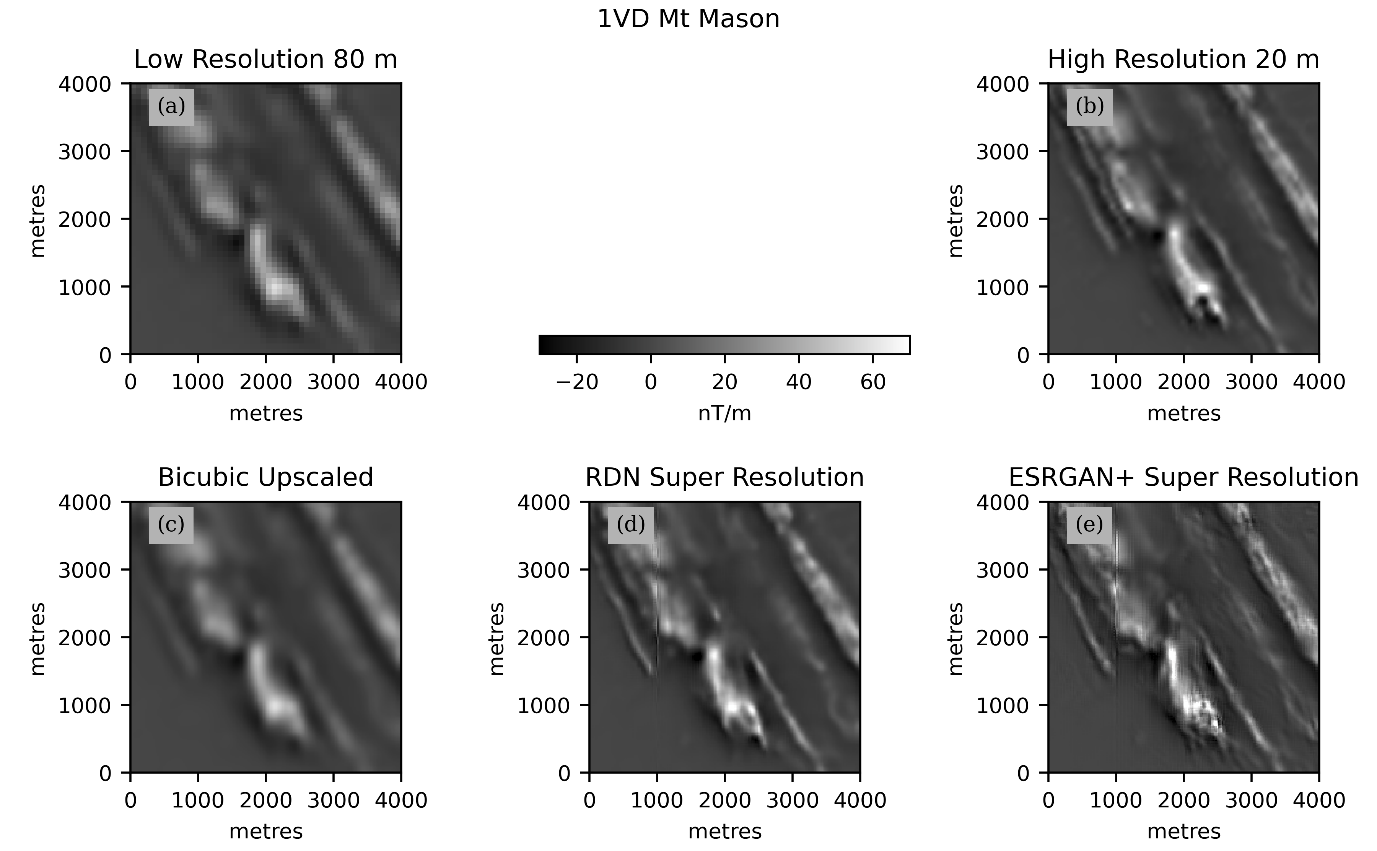
\includegraphics[width=\textwidth]{fig/p1/image9.png}
    \caption[High Pass filtered results]{High Pass filtered test tile and its upsampled counterparts.
    The cut-off for the high pass Butterworth filter was selected with wavelength equal to the Nyquist wavelength of the LR grid, i.e. four times the HR Nyquist wavelength
    }
    \label{fig:filtered}
\end{figure}

\begin{table}
    \begin{tblr}{
        colspec={
            r
            Q[si={table-format=2.3},r]
            Q[si={table-format=2.3},l]
            Q[si={table-format=2.3},r]
            Q[si={table-format=2.3},l]
            Q[si={table-format=2.3},r]
            Q[si={table-format=2.3},l]
            },
        row{1-2} = {guard}
    }
    & Bicubic & & RDN\textdaggerdbl{} & & ESRGAN+ & \\
    \hline{}
    & Mean & {Standard \\ Deviation} & Mean & {Standard \\ Deviation} & Mean & {Standard \\ Deviation} \\
    RMSE   & 13.545 & 26.576 & 7.265 & 13.741 & 11.120 & 21.670 \\
    SISM    & 0.924 &  0.047 & 0.959 &  0.037 &  0.922 &  0.054 \\
    MS-SSIM & 0.971 &  0.018 & 0.988 &  0.012 &  0.976 &  0.020 \\
    \end{tblr}

    \caption[Accuracy Metrics]{
        Accuracy metrics for each upsampling method.
        The best performing method for each metric is bolded.
     }
    \label{tab:metrics}
\end{table}


\subsection{Jasper Hill / Lord Byron super-resolution}
A low-resolution TMI extent from the \SI{80}{\metre} state map over the Jasper Hill major resource project was selected for detailed investigation.
This extent was surveyed at \SI{50}{\metre} (optimal cell size of \SI{10}{\metre}), and is outside of both the defined training and test extents.
A zoomed result for each upsampling method is shown in \cref{fig:jhilldykes}.
The bicubic filter produces a smooth interpolation with limited magnetic intensity enhancement of the features, while both neural network methods produce a more accurate value prediction.
East-West striking features, like those that have been associated with gold mineralisation in the region \parencite[p.~283]{salierTimingSourceGoldbearing2003} are better delineated when using RDN\textdaggerdbl{} and ESRGAN+, and nearly unobservable with bicubic interpolation.
This can be seen in the line profile (\cref{fig:jhilldykes}, f), where a series of East-West striking features have a total magnitude of approximately \SI{100}nT in the low-resolution and bicubic grids, versus approximately \SI{200}nT in the Residual Dense Network prediction and HR groundtruth.
The ESRGAN+ prediction profile shows two distinct low TMI features, but they are poorly located and incoherent in the TMI grid (\cref{fig:jhilldykes} e), which shows an example of the ripple-mark artefact previously noted.

\begin{figure}[hbt]
    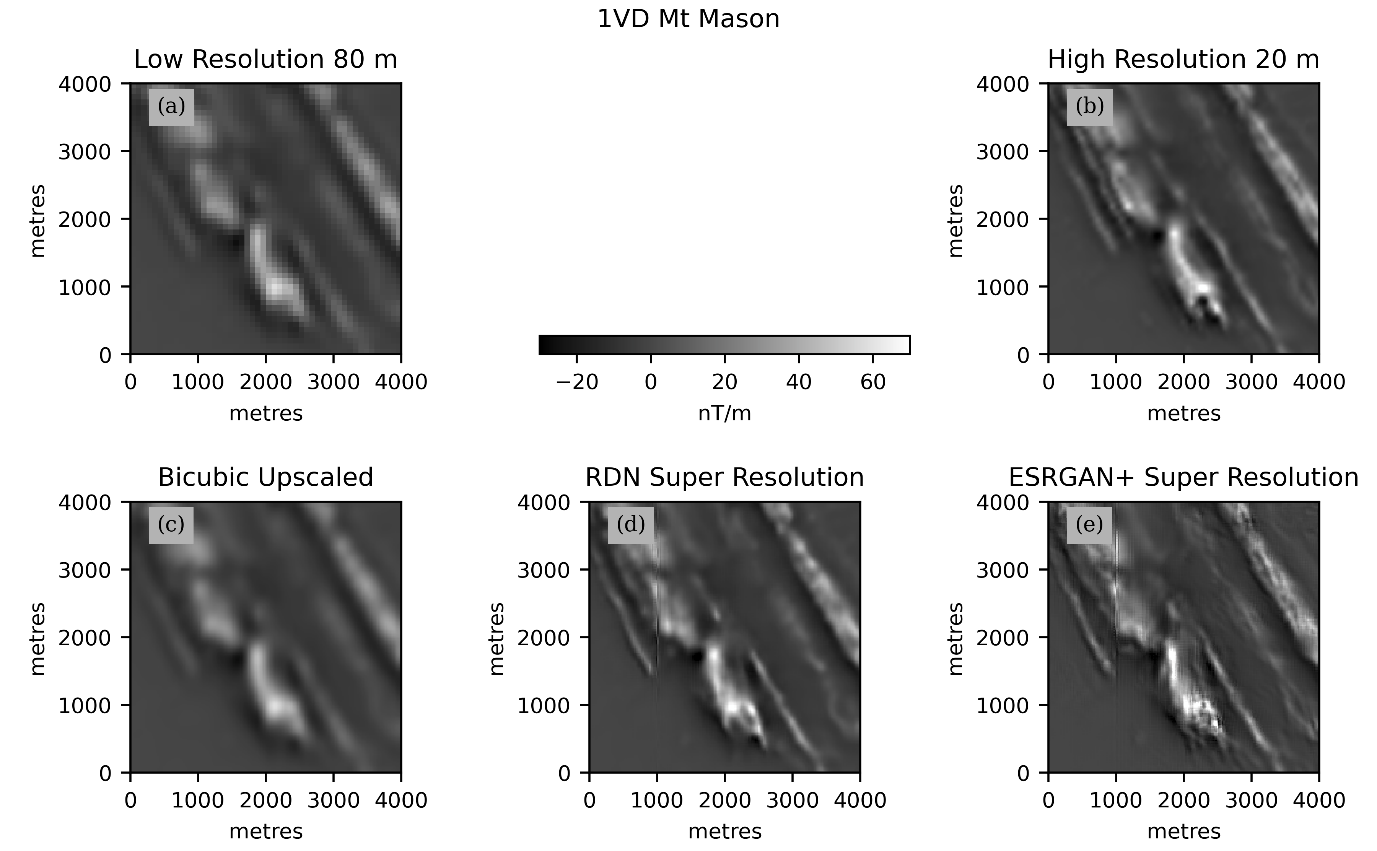
\includegraphics[width=\textwidth]{fig/p1/image10.png}
    \caption[First Vertical Derivative SR TMI over the Mt Mason resource project]{First Vertical Derivative TMI over the Mt Mason resource project, with the super-resolution predictions (d, e) showing a variety of inference artefacts.
    Red asterisks (*) show a vertical tile boundary present as a 3--4 pixel-wide error in predicted TMI value.
    Red caret (\^{ }) indicates a region of subtle ripple-mark textural artefact, only present in ESRGAN+ predictions.
    }
    \label{fig:jhillvis}
\end{figure}

\begin{figure}[hbt]
    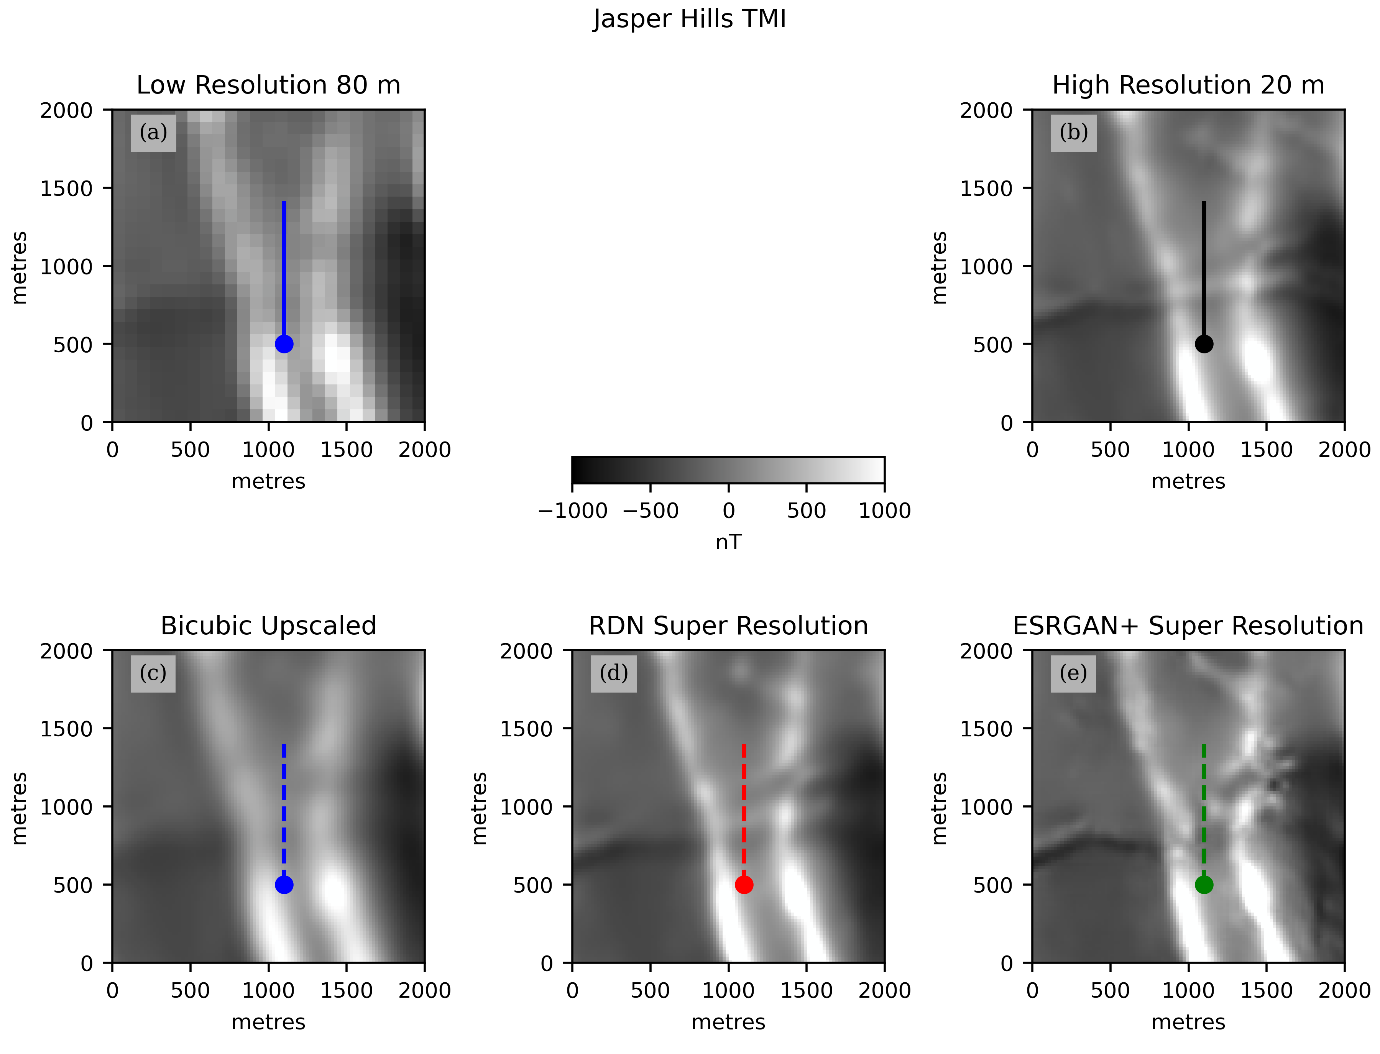
\includegraphics[width=\textwidth]{fig/p1/image11.png}
    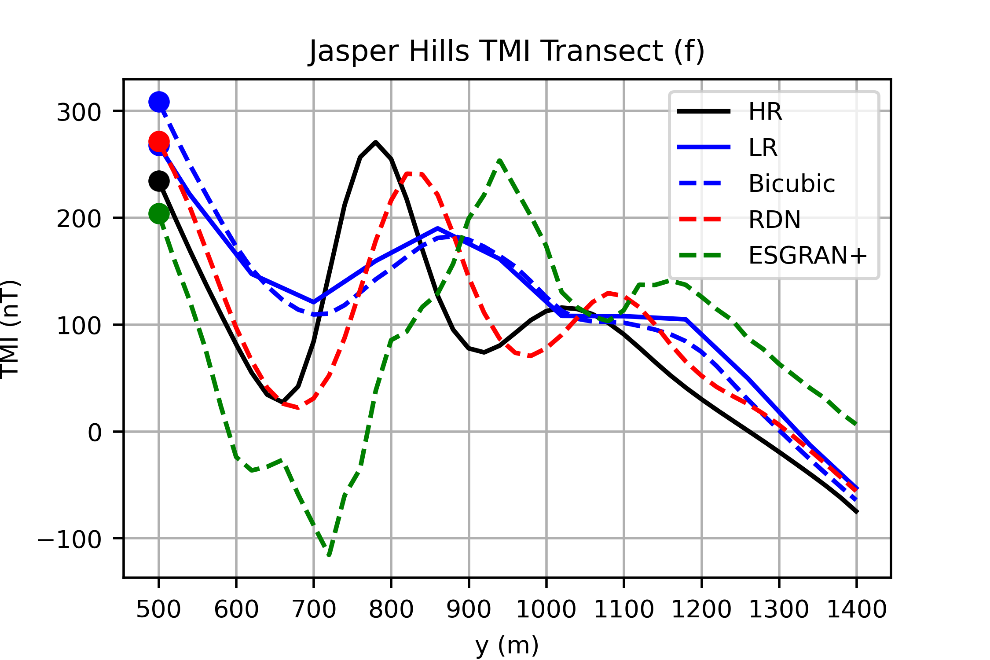
\includegraphics[width=\textwidth]{fig/p1/image12.png}
    \caption[Jasper Hills Project TMI grids and line profile]{Jasper Hills Project TMI grids (a--e) and line profile (f).
    Bicubic interpolation of the low-resolution grid closely matches the low-resolution grid, while both super-resolution methods better approximate the magnitude of the features present in the HR profile, between \SI{650}{\metre} and \SI{1020}{\metre}.
    }
    \label{fig:jhilldykes}
\end{figure}

\section{Discussion}
These results demonstrate that a neural network approach is suitable for high quality super-resolution of geophysics data, surpassing bicubic interpolation in each metric and better resolving structural features.
Importantly, mineralisation controlling structural features that are unresolvable in low-resolution grids become observable in super-resolved grids using a Residual Dense Network.
RDN\textdaggerdbl{} outperforms ESRGAN+ in both accuracy and structural metrics, and most closely visually matches the high resolution groundtruth.
However, ESRGAN+ occasionally appears to better reconstruct features present in the high-resolution ground truth when compared to RDN\textdaggerdbl{}, but at the cost of significant textural noise.
Based on this, RDN\textdaggerdbl{} shows the best performance for super-resolution CNN upsampling of magnetic grids, to assist in the interpretation of low-resolution grids.
The deep learning methods used here can be trained with data from other geospatial extents, either from scratch or by initialising the training with pre-existing model weights \parencite[][e.g.]{wangMineGANEffectiveKnowledge2020}.
The existing models can also be applied to other extents of \SI{80}{\metre} TMI grids without further training.
However, the training data used here are solely \SI{80}{\metre} TMI grids interpolated from high-resolution \SI{20}{\metre} state map extents in the southwest Eastern Goldfields Superterrane.
Magnetic anomalies and features that are dissimilar from those represented in the Superterrane (for example, different geological settings, or regions with different magnetic inclination) are likely to suffer from reduced performance.
This applies also to grids that do not have a cell size of \SI{80}{\metre}.
An example use case for either the method or trained models is super-resolving the Total Magnetic Intensity (TMI) Grid of Australia 2019 - seventh edition which is published by Geoscience Australia in only \SI{80}{\metre} and \SI{40}{\metre} cell size.
The trained \SI{80}{\metre} models in this work could be applied to the \SI{80}{\metre} TMI grid, or the method used with existing state map data to train a two times scale model to super-resolve the \SI{40}{\metre} grid to \SI{20}{\metre}.
Transferability of the model used in this study to other geological settings and magnetic inclinations requires further investigation, with the aim of developing a single multi-domain potential field upscaling model.

The use of the state magnetic map at \SI{80}{\metre} and \SI{20}{\metre} for training data serves as a ready-made analogue for a low pass filter process, which the super-resolution networks successfully learnt to reverse.
While the result presented here demonstrates the strong applicability of performing super-resolution with grids containing magnetic textures and features, it does not yet demonstrate a capability to super-resolve widely spaced line surveys as if they had been surveyed at closer line spacing.
Such grids include artifacts from the gridding process that do not occur in low pass filtered or interpolated high-resolution grids, and will present an additional challenge to super-resolve.
These challenges remain for future work.
Finally, the current models show good performance at a scale factor of \num{4}, which is a typically investigated scale factor in super-resolution research.
Provided with sufficient training data, super-resolution geophysics at other factors would be beneficial, especially targeting typical scale factors between regional and district-scale exploration surveys.

\section{Conclusions}
Convolutional neural network architectures, such as RDN and ESRGAN, are capable of super-resolution upsampling low-resolution magnetic grids into realistic high-resolution grids.
These super-resolved grids contain structural features and textural information that are accurate against ground truth high-resolution grids, that were otherwise unrecoverable through existing interpolation methods.
The method and existing trained models can be applied to other magnetic grid extents, in the Eastern Goldfields Superterrane and beyond.

\section{Declaration of Competing Interest}
The authors declare the following financial interests / personal relationships which may be considered as potential competing interests: This work was supported by a Rio Tinto Iron Ore PhD scholarship.

\printbibliography{}


\end{document}